\subsection{Grafische Oberfläche \raspi}\label{sec:Grafische Oberfläche}
Der \raspi kann nicht nur mit Befehlen über die Befehlszeile bedient werden, sondern auch über eine grafische Oberfläche. Die GUI vereinfacht zum Beispiel die Implementation von Daten, ermöglicht einen Remote-Zugriff und kann bei der Entwicklung von Anwendungen hilfreich sein.\\
\vspace{3mm}
\begin{figure}[htbp]
    \centering
    \begin{subfigure}[b]{0.45\textwidth}
        \centering
        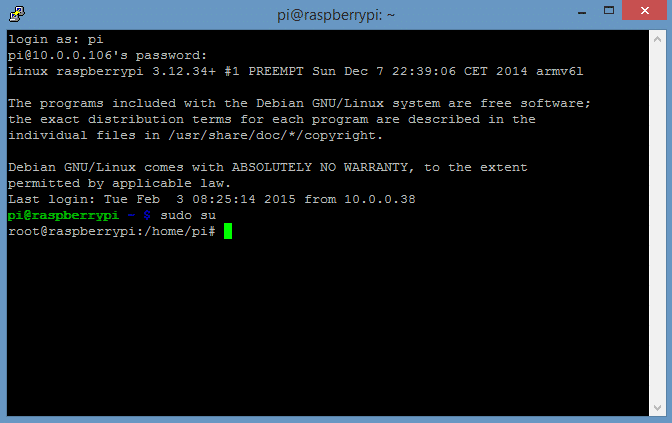
\includegraphics[width=\textwidth]{image/terminal.png}
        \caption{Befehlszeile}
        \label{fig:bild1}
    \end{subfigure}
    \hfill
    \begin{subfigure}[b]{0.5\textwidth}
        \centering
        \includegraphics[width=\textwidth]{image/pixeloberfläche.jpg}
        \caption{grafische Oberfläche}
        \label{fig:bild2}
    \end{subfigure}
    \caption{Befehlszeile\autocite{Befehlszeile}  und grafische Oberfläche\autocite{Grafische-Oberfläche}}
    \label{fig:zwei_bilder}
\end{figure}
\vspace{3mm}
Die grafische Oberfläche kann mit wenigen Befehlen installiert werden. \\
Als erstens wird der X-Server installiert. Dieser Server ist die Grundlage um grafische Oberflächen zeichnen zu können.\\
\vspace{3mm}
\begin{verbatim}
sudo apt-get install --no-install-recommends xserver-xorg xinit
\end{verbatim}
\vspace{3mm}
Nachdem der X-Server installiert wurde, kann die Desktopumgebung heruntergeladen werden. Es gibt viele verschiedene Umgebungen. Die Pixel Umgebung ist eine Desktop-Umgebung und wurde speziell auf den \raspi angepasst und eignet sich somit sehr gut für diese Anwendung.\\
\vspace{3mm}
\begin{verbatim}
sudo apt install raspberrypi-ui-mods
\end{verbatim}
\vspace{3mm}
Bevor der \raspi neu gestartet wird, kann in der Konfiguration noch eingestellt werden, ob der \raspi vor dem Starten nach einem Passwort fragen soll oder nicht.\\
Mit dem unten angegebenen Befehl wird die Konfiguration\autocite{raspberry_Konfiguartion} geöffnet.
\vspace{3mm}
\begin{verbatim}
sudo raspi-config
\end{verbatim}
\vspace{3mm}
Nachdem diese Wahl getroffen wurde, kann der \raspi neu gestartet werden und beim nächsten Starten wird die grafische Oberfläche sichtbar.
\subsection{Remote-Zugriff}\label{sec:Remote Zugriff}
Um auf den \raspi zuzugreifen, auch wenn dieser nicht am selben Standort ist, wird ein Remote-Zugriff eingerichtet. Durch einen Remote-Zugriff, können Benutzer auf entfernte Geräte zugreifen. Es gibt eine Vielzahl von Protokollen die einen Remote-Zugriff ermöglichen. Die am häufigsten verwendeten Protokolle sind:
\begin{itemize}
  \item Remote Desktop Protocol (RDP)
  \item Virtual Network Computing (VNC)
  \item Secure Shell (SSH)
\end{itemize}
\vspace{3mm}
Das Secure Shell Protokoll auch SSH genannt, sorgt für eine sichere Verbindung zwischen zwei Geräten. Das Protokoll baut eine verschlüsselte Verbindung auf und ist ebenfalls dafür zuständig, dass Daten die an den Empfänger gesendet werden, nicht manipuliert werden. Um eine SSH Verbindung aufzubauen  benötigt man die Anmeldedaten und eine Schnittstelle. SSH bietet eine  Kennwortauthentifizierung mit hoher Sicherheit. Es können aber auch andere Authentifizierungsmöglichkeiten verwendet werden. Die Schnittstelle kann das Terminal aber auch integrierte Optionen in VS-Code sein.\\
\vspace{3mm}
\begin{wrapfigure}{r}{7cm}
  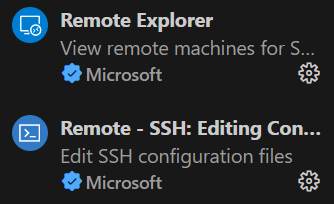
\includegraphics[scale = 1.2]{image/Erweiterungen.png}
  \caption{Erweiterungen in VS-Code}
\end{wrapfigure}
In VS-Code gibt es eine Erweiterung um einen Remote-Zugriff zu ermöglichen. Die Erweiterung \textbf{Remote-SSH} muss installiert werden, da diese nicht Standardmäßig in VS-Code vorhanden ist. Der \textbf{Remote Explorer} zeigt an, mit welchem Gerät der Laptop schon verbunden war oder mit welchen Geräten eine Verbindung aufgebaut werden kann.\\
\newpage
Im Remote Explorer kann ein neues Gerät hinzugefügt werden. 
\begin{itemize}
  \item mit dem New Remote wird ein Gerät hinzugefügt.
  \item Danach wird der Name des \raspi und die IP-Adresse angegeben. Zum Beispiel:
  \begin{verbatim}
jusch@192.168.10.34
\end{verbatim}
  \item Nach diesem Schritt wird das Passwort abgefragt. 
  \item Wenn diese Schritte erfolgreich waren, wird eine SSH-Verbindung aufgebaut.
\end{itemize}
